\section{Operation Governance and Evidence}
\label{sec:modules}
Section~\ref{sec:design} defines the shared dispatch contract. This section
focuses on the checks that follow it: scene-specific write admission,
conditional approval, and the records returned by each route.

\subsection{Scene-Specific Write Admission}
\label{sec:governed}
After the shared dispatch checks pass, the selected handler applies the
limits configured for the target scene and control. Authorization and value
admission are separate checks. The target band describes a desired process
outcome; it does not define the admissible write interval. A candidate may
satisfy all write constraints while the measured process value remains outside
the target band.

For an online node write, the admissible value interval is
\begin{equation}
\mathcal{I}^{\mathrm{online}}_n(t)=
\mathcal{H}_n\cap\mathcal{L}^{\mathrm{base}}_n\cap\mathcal{L}^{\mathrm{prod}}_n(t)\cap\mathcal{L}^{\mathrm{rec}}_n(t),
\label{eq:admission}
\end{equation}
where $\mathcal{H}_n$ is the hard engineering range, and
$\mathcal{L}^{\mathrm{base}}_n$, $\mathcal{L}^{\mathrm{prod}}_n$, and
$\mathcal{L}^{\mathrm{rec}}_n$ are the baseline, active-product, and
active-recipe limits. These numerical bounds are distinct from the scope,
policy, grant, and binding predicates in Eq.~(\ref{eq:dispatch-contract}).
Missing optional limits impose no restriction. An empty intersection rejects
the request and identifies the excluding layer. Recipe dispatch checks a
replacement recipe against the hard, baseline, and product limits rather than
the previous recipe's window. Step, interval, and hold-window limits apply
when configured. These application-level checks complement, but do not
replace, equipment interlocks.

\begin{figure}[!t]
\centering
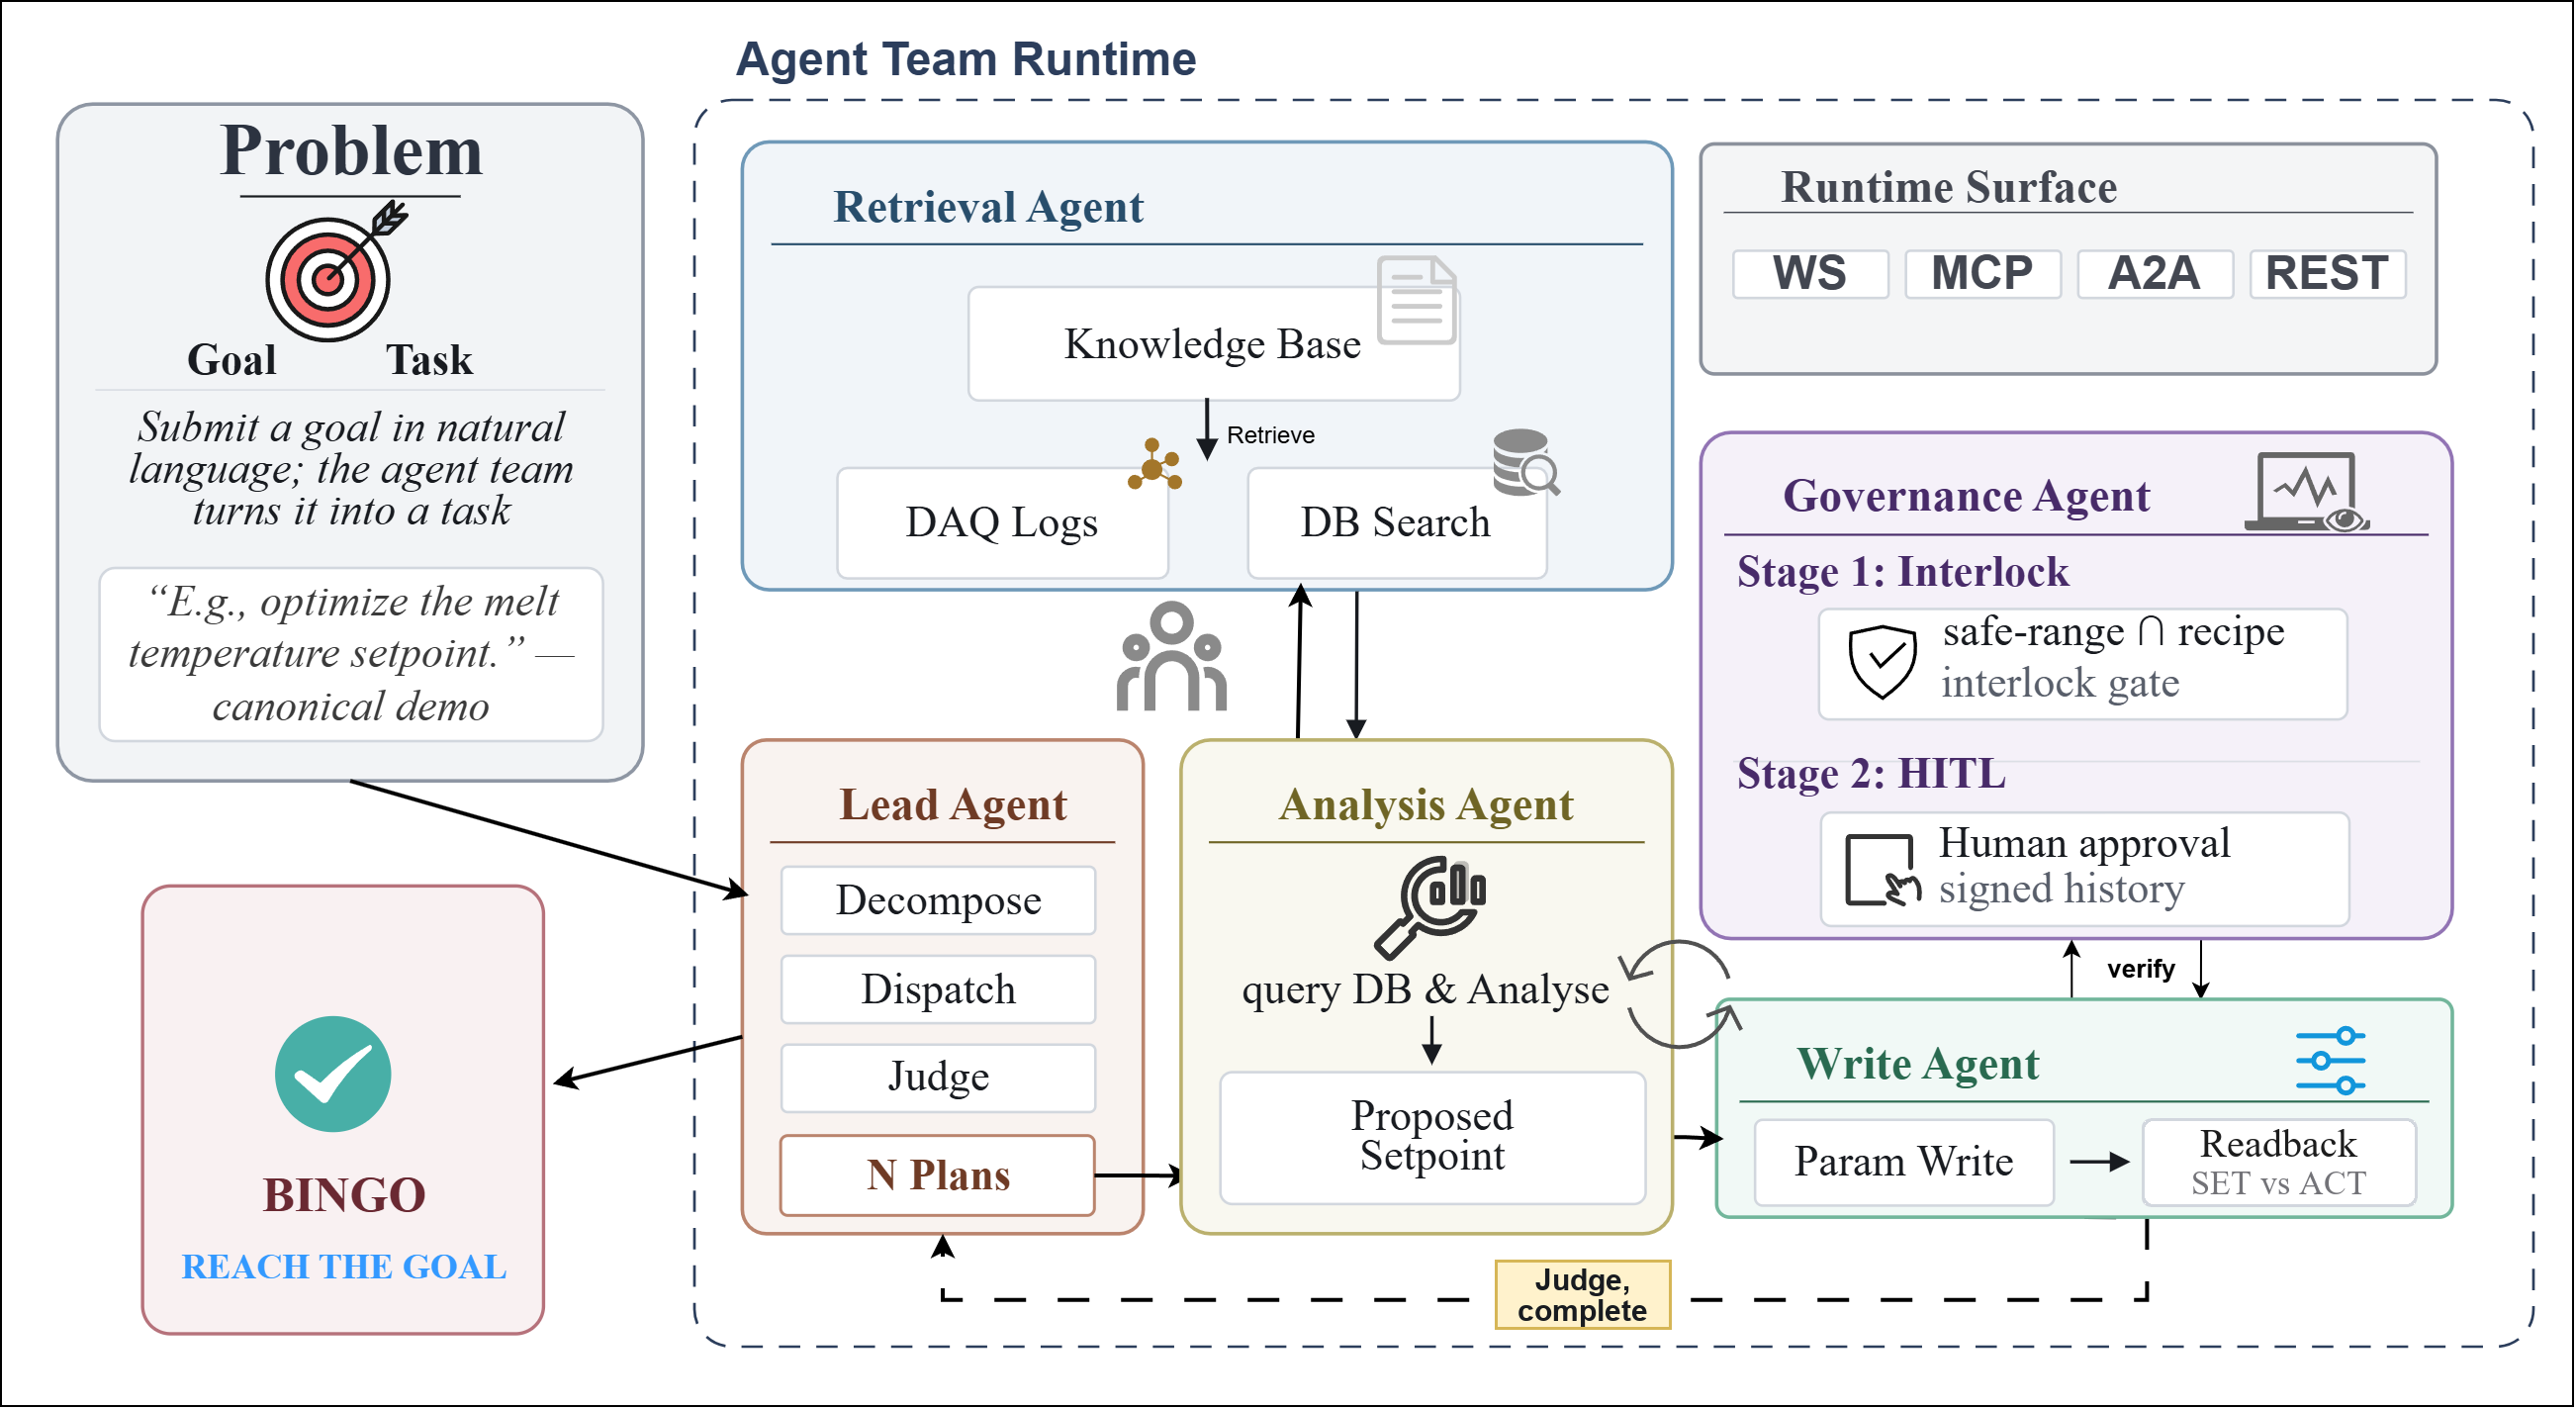
\includegraphics[width=\columnwidth]{resources/aws_fig3-flat.png}
\caption{Implemented agent-team runtime. A natural-language goal enters as
a task; the lead agent decomposes and dispatches plans; retrieval and
analysis produce the proposed setpoint (the LLM engine occupying a
replaceable strategy slot). The governance stages are deterministic platform
logic: Gate~1 applies the Eq.~\eqref{eq:admission} interlock, Gate~2 the
approval wait; the write agent reads back the value actually present (SET
versus observed ACT), and the judge records keep, rollback, or uncertain;
every step is journaled with actor attribution. The block labeled
``Governance Agent'' denotes these deterministic platform stages, not a
model-bearing agent; the judge annotation is the caller's verdict-tool
invocation.}
\label{fig:runtime}
\end{figure}

\section{Governed Execution Mechanisms}
\label{sec:mech}
A supervisory intervention must preserve distinctions that an agent tool call
usually collapses---permission to propose, admission of a value, driver
acceptance, device confirmation, process response, a caller's verdict, and
compensation---and \system{} exposes these as separate evidence states.
Three design commitments generate that separation: model output is treated
as an untrusted proposal, never as authority; evidence is graded by what is
observed rather than by what was claimed; and failure states are surfaced
for inspection rather than absorbed into a success flag.
Fig.~\ref{fig:runtime} shows the implemented agent-team
runtime that carries these steps; the governance and write stages drawn in
the figure are deterministic platform logic---no model output can admit,
approve, or confirm a write (Gates~1--2 of Fig.~\ref{fig:runtime}). A governed intervention is
one transaction in the audit-trail sense: every step
leaves its own evidence record, while execution and recovery are deliberately
not atomic with device state (Section~\ref{sec:limits}).
Six invariants organize the path---binding-resolved authority (never channel
membership or prompt content), Eq.~\eqref{eq:admission} admission,
fail-closed approval waits on manual bindings, graded rather than
success-flag acknowledgment, checkable three-way consistency, and
separately admitted compensation---each specified in the subsections that
follow, and every agent-originated path to the plant passes through the
same governed write.

\begin{figure}[!t]
\centering
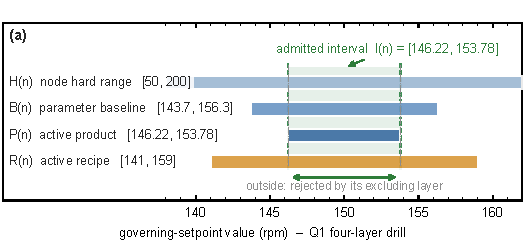
\includegraphics[width=\columnwidth]{resources/fig-admission.pdf}
\vspace{1pt}
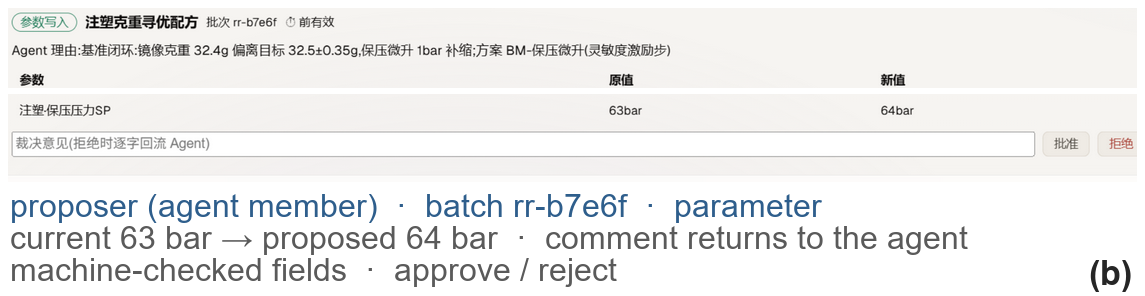
\includegraphics[width=0.78\columnwidth]{resources/hitl-card-crop.png}
\caption{The admission boundary and its human-approval gate, on the running
benchmark line. (a)~The Eq.~\eqref{eq:admission} interval geometry: four declared,
versioned bounds narrow to the admitted interval; a proposal
outside it is rejected by its excluding layer (the Q1 four-layer drill).
(b)~The structured approval card on a manual binding (live system, gloss
added): machine-checkable fields are separated from the proposer's
display-only reasoning; the comment returns to the member on refusal
(Section~\ref{sec:hitl}).}
\label{fig:hitl}
\end{figure}

\subsection{Task, Observation, and Admission}
\label{sec:objective}
The strategy receives a task and goal in production context and decides what
to propose and when to stop; the platform governs execution over semantic node
parameters---pressure, dosing rate, line speed, rail
width---in engineering units.

\looseness=-1 For an ordinary agent setpoint request on node $n$, the
admission interval is
\begin{equation}
\mathcal{I}_n(t)=\mathcal{H}_n\cap\mathcal{B}_n
                 \cap\mathcal{P}_n(t)\cap\mathcal{R}_n(t),
\label{eq:admission}
\end{equation}
where $\mathcal{H}_n$ is the mandatory hard engineering range (finite and
non-empty at node creation) and the remaining terms the baseline,
active-product, and active-recipe limits; a missing optional limit
contributes no restriction, so the interval is always defined, and $t$ is the
admission instant, re-resolved at execution. Should a configuration empty the
intersection, every write is rejected with the excluding layer named, so the
misconfiguration surfaces at the first write. The interval form is
deliberate: every bound is a declared, versioned object that an audit can
replay against the active product and recipe, and rejection is decidable and layer-attributable, where a learned
feasibility model offers neither
(Fig.~\ref{fig:hitl}a)---a decidability claim, not a safety certificate.
It bounds one parameter at a time---joint,
cross-variable windows live in scenario guards---and bounds magnitude, not
intent: availability, binding state, and approval policy are checked
separately, and in-window but adverse sequences surface at verdict and
compensation (Section~\ref{sec:scenarios} reports two).

\subsection{Semantic Write, Pacing, and Source-Specific Routes}
\label{sec:nodeexec}
A semantic card exposes quantity, unit, precision, range, value, freshness,
and recipe context; the controller resolves binding and limits, the driver
serializes the command, and the acknowledgment grade closes the
command path, never the process-response path (Section~\ref{sec:ack}). Two write-spacing windows pace governed loops, never
the plant: online writes---agent- or human-origin---sit at least 60\,s apart
with a hold window after success (HTTP~429 inside it); a per-recipe dispatch
interval anchored at the \emph{approval} instant is restart-persistent, so
alternating identities cannot reset it; and a 300\,s per-line trial cadence
damps same-line trials from any origin. Recipe-dispatch and rollback writes
are exempt. \texttt{AW\_BENCH\_MODE=1} admits harness-declared arms that
relax the soft window or readback---never the hard range.

\looseness=-1 Four governed routes---agent tools, human-origin writes, recipe
dispatch, and rollback compensation---reach the same driver through one
admission and journaling entry point, the hard range included; recipe
dispatch adds run context---the line-scoped execution window, the reduced
ISA-88 batch/lot notion---validated at save time. Hold heartbeats (periodic
re-dispatch of the stored setpoint) are the one non-governed re-dispatch:
off by default, stopped by line stop or driver change, and re-applying the
stored value without re-admission---plant-facing state maintenance, not an
agent path. Line start installs active context before recipe parameters
dispatch individually, and line stop clears it; these multi-step operations
are not atomic with device state.

\subsection{Write Acknowledgment as Three-Level Evidence}
\label{sec:ack}
A driver-level success flag conflates two facts: the transport
accepted the command, and the device now holds the value. \system{} grades
every governed write into one of three acknowledgment levels:
\emph{readback-verified} when an independent read---one issued outside the
write path---returns the commanded value within the node's configured write
tolerance;
\emph{transport-acknowledged} when the transport
accepted the command on an endpoint with no usable readback;
\emph{unverified} when the transport failed or when post-write verification
could not confirm the value. The grading rule is falsifiable. Under a
success-flag receipt rule---a transport acknowledgment closes the
report---the publish-only receipt demonstrated in
Section~\ref{sec:hardening} (broker puback, \texttt{ok=true}, no read
channel, three verification attempts) reports \emph{success}; the graded
rule reports it \emph{unverified}. That is what fail-honest means: absence
of evidence degrades the grade, never the report, and the grade is fixed
when the write closes.

A transport-acknowledged write may still not have reached the device, so a
post-write verifier re-reads the endpoint (three attempts, 2\,s apart) and
promotes the grade when a read confirms the value. Batch receipts carry a
per-parameter grade plus a summary; the write journal stores the per-write
grade, and the operations log records the judgment at worst-state
severity. Recipe rollback restores a definition,
not physical PLC values, and a compensating write is itself graded by the same
three levels. The grade closes the command path only: readback-verified says the device
holds the value, not that the process responded as intended---that
distinction belongs to observation and verdict.

\subsection{Observation, Verdict, and Compensation}
\label{sec:agentloop}
\looseness=-1 An agent- or rollback-source write opens an optimization record;
the verdict tool
\texttt{dcw\_judge} records \texttt{keep}, \texttt{rollback}, or
\texttt{uncertain} plus a reason; the verdict, stored with the record it closes
and the response window actually queried, performs no actuation and does not
independently validate the evidence, so a scripted keep can coexist with a
missed objective---verdict integrity rests on attribution, journaling, and
operator review: a kept-but-marked record stays visible with its
disagreement attached, and the operations log raises parameter severity
under alarm-rationalization practice (Section~\ref{sec:limits}). Three-way
setpoint consistency is checked by the evaluation harness rather than the
platform: the harness compares the recipe
value, the device readback, and a mirror sample
drawn from the acquisition runtime's separate polling path and store, each leg
against a stated tolerance; the sampled legs meet at the plant endpoint, so a
fault fabricating the endpoint is a common-mode boundary.
Disagreement fails the harness check and is reported with the run. Verdicts are attributable---actor and timestamp travel
with them, and corrections amend the stored reason visibly.

Compensation is a new, separately admitted write that may fail or partially
complete; it is graded by the Section~\ref{sec:ack} levels, and a rollback
record settles to rolled back once the compensating write is
accepted---readback-verified where the endpoint supports readback,
transport-acknowledged otherwise. If the compensating write is itself
refused by admission, the source record closes \emph{as judged}, with the
refusal appended to its verdict. These separations keep command status,
record status, and process recovery independently inspectable.

\looseness=-1 The backstop is a record-integrity check for writes that no
verdict has closed---not an independent protection layer: it evaluates only
open records; a caller's \texttt{keep} closes the record and stands it down,
while a \texttt{rollback} verdict stands the backstop down only once the
compensating write executes---so its availability is contingent on verdicts
being recorded and observations arriving. When collected samples of an open
record's node leave the recipe's monitoring window (a DAQ-side envelope
distinct from the admitting interval), the platform issues a
system-attributed rollback verdict and restores the value preceding that
write (one step; the admitted baseline is not restored), graded as above.
The policy waits 120\,s, polls every 30\,s, and fires on three
out-of-window samples---cumulatively, not necessarily consecutively;
non-returning samples count no breach, so an acquisition outage leaves the
record open and unalarmed. Recovery runs only while fewer than two retained
rollback records stand on the node, past which the backstop judges but
defers actuation to the governing approval policy.

\subsection{Human Approval Boundary and the Line Master Switch}
\label{sec:hitl}
\looseness=-1 Manual bindings insert the timed approval wait before
an agent setpoint or
compensation request; automatic bindings omit the wait but keep the checks.
The pending request shows member, node, value, interval, and expiry---in the
deployed benchmark, plus the proposer's reasoning and per-parameter basis
(Fig.~\ref{fig:hitl}b): machine-checked fields are structured data, the
free-text reasoning display-only and non-authoritative. Because binding and admission are
re-checked at execution, approval reserves neither interval nor device state;
the approval dialog---itself an injection surface (Section~\ref{sec:limits})---
cannot promote a proposal past the checks; the comment returns verbatim
to the proposing member on refusal and travels with the receipt on
approval---feedback, not authority. The
wait fails closed by default (expiry 180\,s): an expired request
resolves as refusal and is recorded; duplicates are suppressed by holding
one pending request per member--node pair; and in \emph{hold} mode an
unanswerable request persists without expiry until a human answers, with
repeat requests refused as duplicates.

Human authority is anchored one level above individual requests: each line
carries a control mode---the line master switch---whose fail-safe default
is \emph{manual}. Under manual
mode, recipe-family operations (parameter update, dispatch, trial, and
rollback) from approval-free bindings on that line are intercepted and
presented for approval regardless of binding policy; direct node-tool
writes remain gated by their binding mode and the admission interval, not
by the line switch. Switching a line
to automatic requires an explicit, admin-only user-side
confirmation---agent identities cannot touch the line switch. The residual
agent-side path is delegation: a lead agent can grant held nodes to a
worker through an attributed lead-only tool, and the grant's execution mode
is chosen at grant time rather than gated by the user-side confirmation;
grants are attributed to the granting agent, cannot exceed its own node
face, and are individually revocable (Section~\ref{sec:limits}).

The decision endpoint authenticates a user but does not enforce a line-scoped
approver role---the gap Section~\ref{sec:limits} carries---and reads,
verdict recording, and some configuration changes do
not use physical-write approval---workflow mediation, not segregation of
duties; a recipe switch between approval and execution re-admits the value
against the new window (Section~\ref{sec:limits}).
The strategy engine is replaceable rather than trusted as a control
primitive: scenario code declares and configures but never executes plant
I/O, and the platform never infers a process objective.

